\section{Graph Families}

When choosing test sets for Dijkstras Single-Source Shortest Paths that hopefully will exhibit different running times based on the performance of the underlying heaps DecreaseKey running time it is important to maximize the difference in the amount of edges.
In order to do this, we wish to chose one test set that is very sparse, and one that is very dense.

\subsection{Sparse Graph}
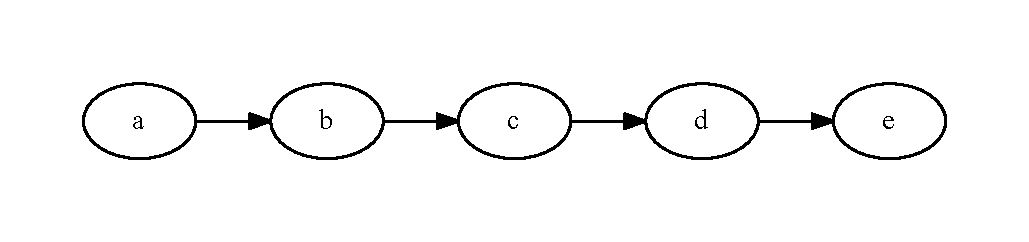
\includegraphics[width=\textwidth]{sparsegraph.pdf}
As our sparse graph, we chose a line of nodes, where each node has both in and out degree of 1, except for the source, which has in-degree 0, and the end, which has out-degree 0. Such a graph will have $O(n)$ edges, and will in fact contain the minimal amount of edges required to keep the graph fully connected.

Alternatives to this graph could be a cycle of nodes, any directed tree, or a star graph, with edges going out from the center nodes.

\subsection{Dense Graphs}
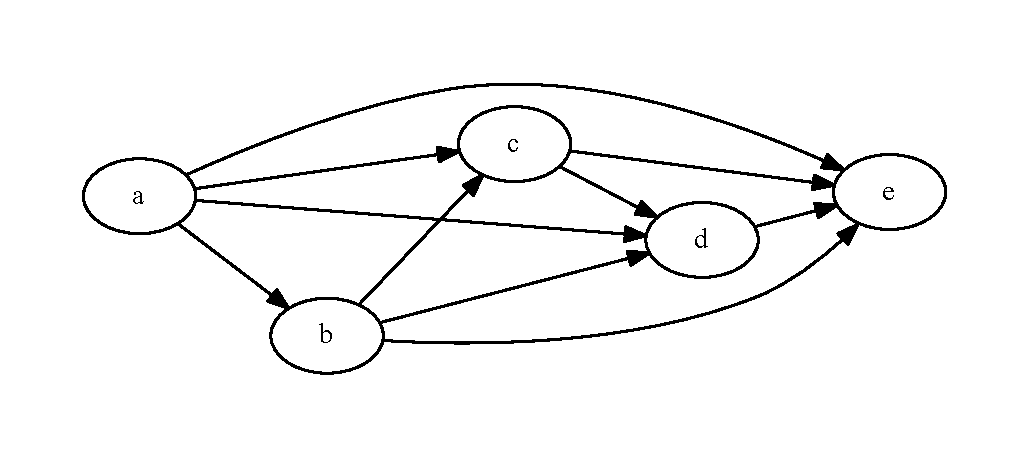
\includegraphics[width=\textwidth]{densegraph.pdf}
As our dense graph, we have chosen a modified version of our sparse line of nodes, where each node has had an outgoing edge to every node in its transitive closure that it did not already have an outgoing edge to added. Such a graph will contain $O(n^2)$ edges. Note that we could add even more edges to this graph, but since Dijkstra's algorithm will not call DecreaseKey for already visited nodes, we would not increase the amount of calls to DecreaseKey.

An alternative to this graph could have been complete digraph, to fully maximize the amount of edges.

